\chapter{相关工作介绍}

\section{人类感光系统原理}
由于近年来蓬勃发展的神经形态视觉传感器追根溯源是受到了人类感光系统的启发,所以有必要讲解一下人类感光系统的原理,并随后分析这种原理如何被创造性地抽象化,利用和改进,以表现出和传统曝光相机在采样机制和数据结构上迥然不同的特点和成像高动态范围的优势。
\subsection{人类感光系统}
人类感光系统是多种细胞组成不同生理结构的有机结合,其核心为视网膜。如图\ref{fig:human_eye}所示,视网膜是一个由多种细胞组成的结构,是位于人眼眼球内侧的高度复杂的精细感光结构。从外层到内层分布着光感受器细胞外段层,包含视锥细胞和视杆细胞的外核层,外网状层,包含水平细胞和双极细胞的内核层,内网状层和向神经中枢传递神经信号的神经节细胞。正因为这些细胞的层次化有序排列,才能使得人眼拥有高分辨率,高动态范围的特性。这为神经形态视觉传感器提供结构和功能上的借鉴。

视网膜感光层的核心是视锥细胞和视杆细胞,它们将光信号转变为人脑可接受处理的电信号。视锥细胞对强光敏感,负责颜色识别,在中央凹区域尤为密集,也恰好是光线入眼的直接接受区域。视杆细胞对弱光敏感,负责照度识别,广泛分布在视网膜外围,构成全眼照度识别的基础。双极细胞处于更深层,接受上述两种细胞反馈的信号,根据光感受野的区域分成“开”、“关”两种形态。水平细胞横亘在外网状层,负责信息之间的传递,调节整体亮度并强化画面视觉边缘。

上述的人眼成像原理,为神经形态视觉传感器的研发提供了理论基础和灵感来源。通过对各种细胞的功能抽象和电子元件功能替代,我们可以设计出具有不同特性和优势的神经形态视觉传感器。
\begin{figure}[ht]
  \centering
  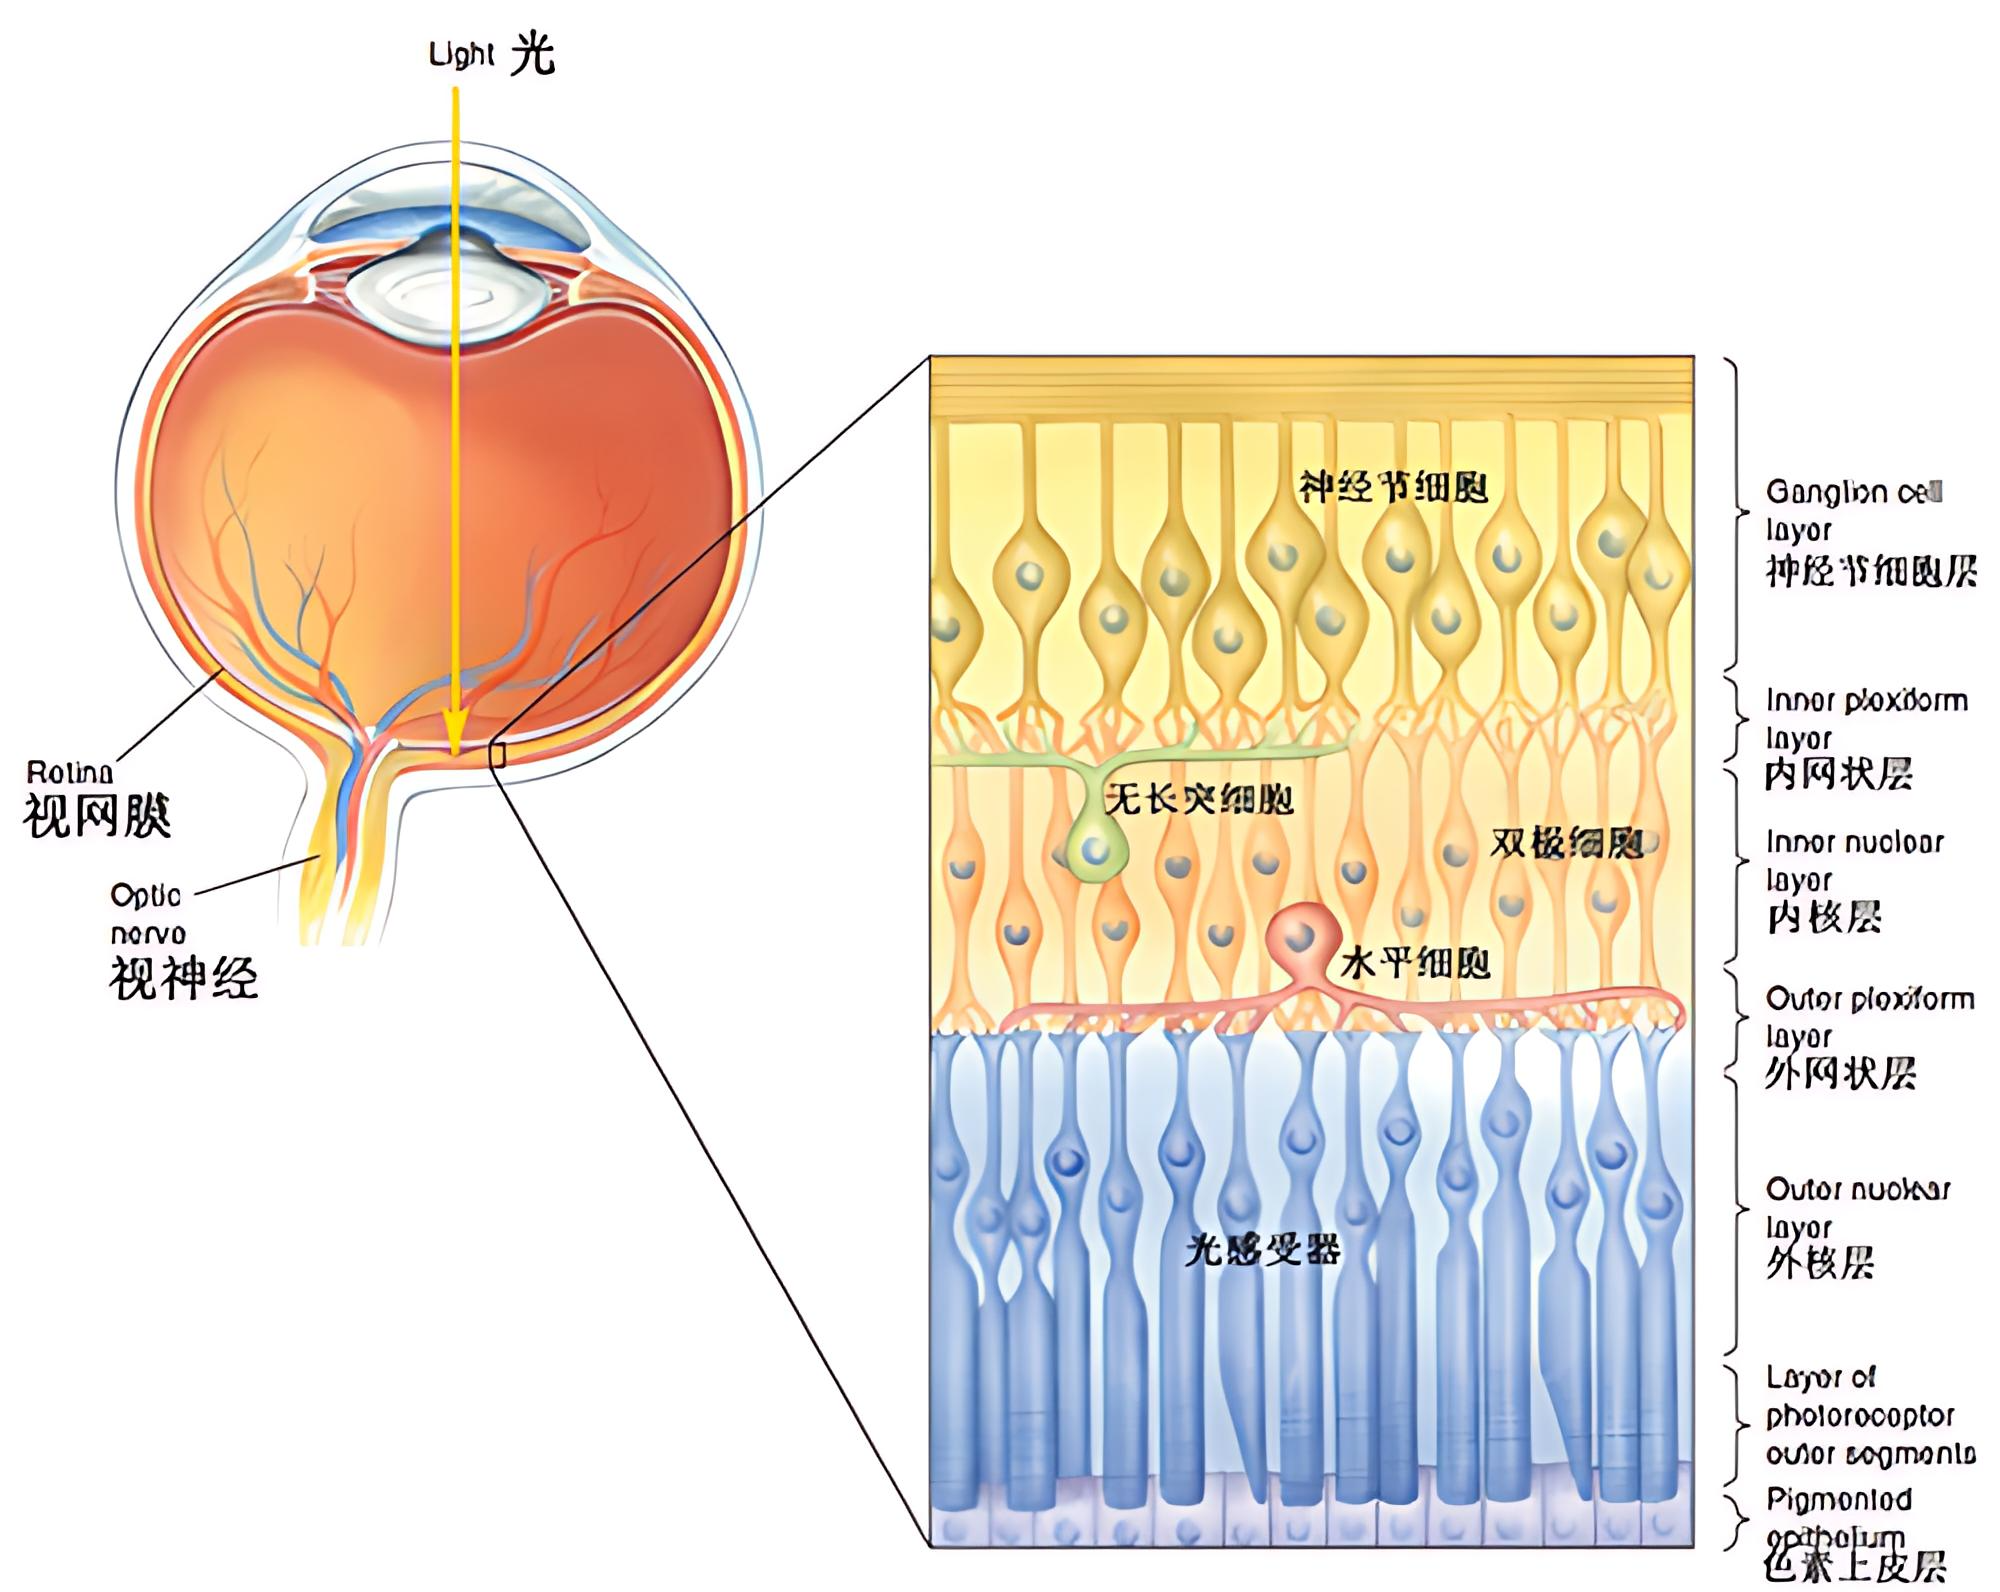
\includegraphics[width=\textwidth]{human_eye.png}
  \caption{人眼及其视网膜结构示意图}
  \label{fig:human_eye}
\end{figure}


\subsection{上述系统对脉冲相机的启发}
来自北京大学的Huang教授及其团队于2018年提出了仿视网膜中央凹采样模型(Fovea like Sampling Model,FSM)\cite{7923720}。此模型借鉴了上述人眼成像机制中视网膜中央凹的感知结构,突出其光敏优势,通过脉冲发放频率和脉冲宽度对光强进行积分,且由于自然界中光强客观存在,脉冲必定发放,通过人为或自适应设定脉冲发放阈值调节“光敏度”保持合理的脉冲密度,籍此避免了传统曝光相机在过暗和过亮情况下无法记录信息的问题。Huang教授及其团队进一步具象化上述原理,自主研发脉冲相机(Spike Camera),采用脉冲序列\cite{dong2018spike}形式传输数据,即高速脉冲帧。随后该团队在时间分辨率和空间分辨率上对硬件开展进一步的提升。表列出了两代Spike Camera的各项详细参数。

\begin{table}
    \centering
    \caption{Spike Camera的各项详细参数}
    \label{tab:spike_camera_parameter}
    \begin{tabular}{ccc}
      \toprule
      Spike Camera & -Gen1\cite{dong2018spike}&-Gen3\cite{Huang_Tiejun110} \\
      \midrule
      年份 &2018&2020 \\
      空间分辨率(像素数) &400\times250&1000\times1000   \\
      时间分辨率($\upmu$s) &50&25    \\
      动态范围(dB) &>110&>110 \\
      最大数据通量(eps) &2G&40G   \\
      芯片尺寸(mm\textsuperscript{2}) &10\times6&20\times20    \\
      像素尺寸(平方毫米)&20\times20&17\times17 \\
      芯片制造工艺(nm) &110&110   \\
      芯片工作电压(V) &12&12    \\
      填充系数 &13.75\%&13.75\% \\
      芯片功耗(mW) &370&3000   \\
      数据接口 &USB3.0&USB3.0    \\
      \bottomrule
    \end{tabular}
  \end{table}

\section{脉冲相机工作原理}